\subsection{Vision Transformer (ViT)}
\label{appendix:vision_transformer}

Vision Transformer \cite{vision_transformer} (ViT) model by Google uses transformer to classify images. Although vision transformer is not categorically a video synthesis model, its important to understand what is it and how it works, since a lot of the text-to-video models rely on the foundation of the paper. ViT only uses the encoder part of the transformer model.

Traditionally CNNs are used to extract local spatial features from an image. However they often fail to capture long-range dependencies (for example the first pixel and the last pixel in the image are very far apart).

One solution is to use transformers's attention mechanism which enable to capture global context of the image (between patches, because of the positional encodings). The Vision Transformer model is composed of two parts: the patch embedding and the transformer encoder.

In their paper, they found that ViT scale more effectively for visual recognition than traditional convolutional networks. The scaling behavior of transformers is better than that of CNNs.

\begin{figure}
    \centering
    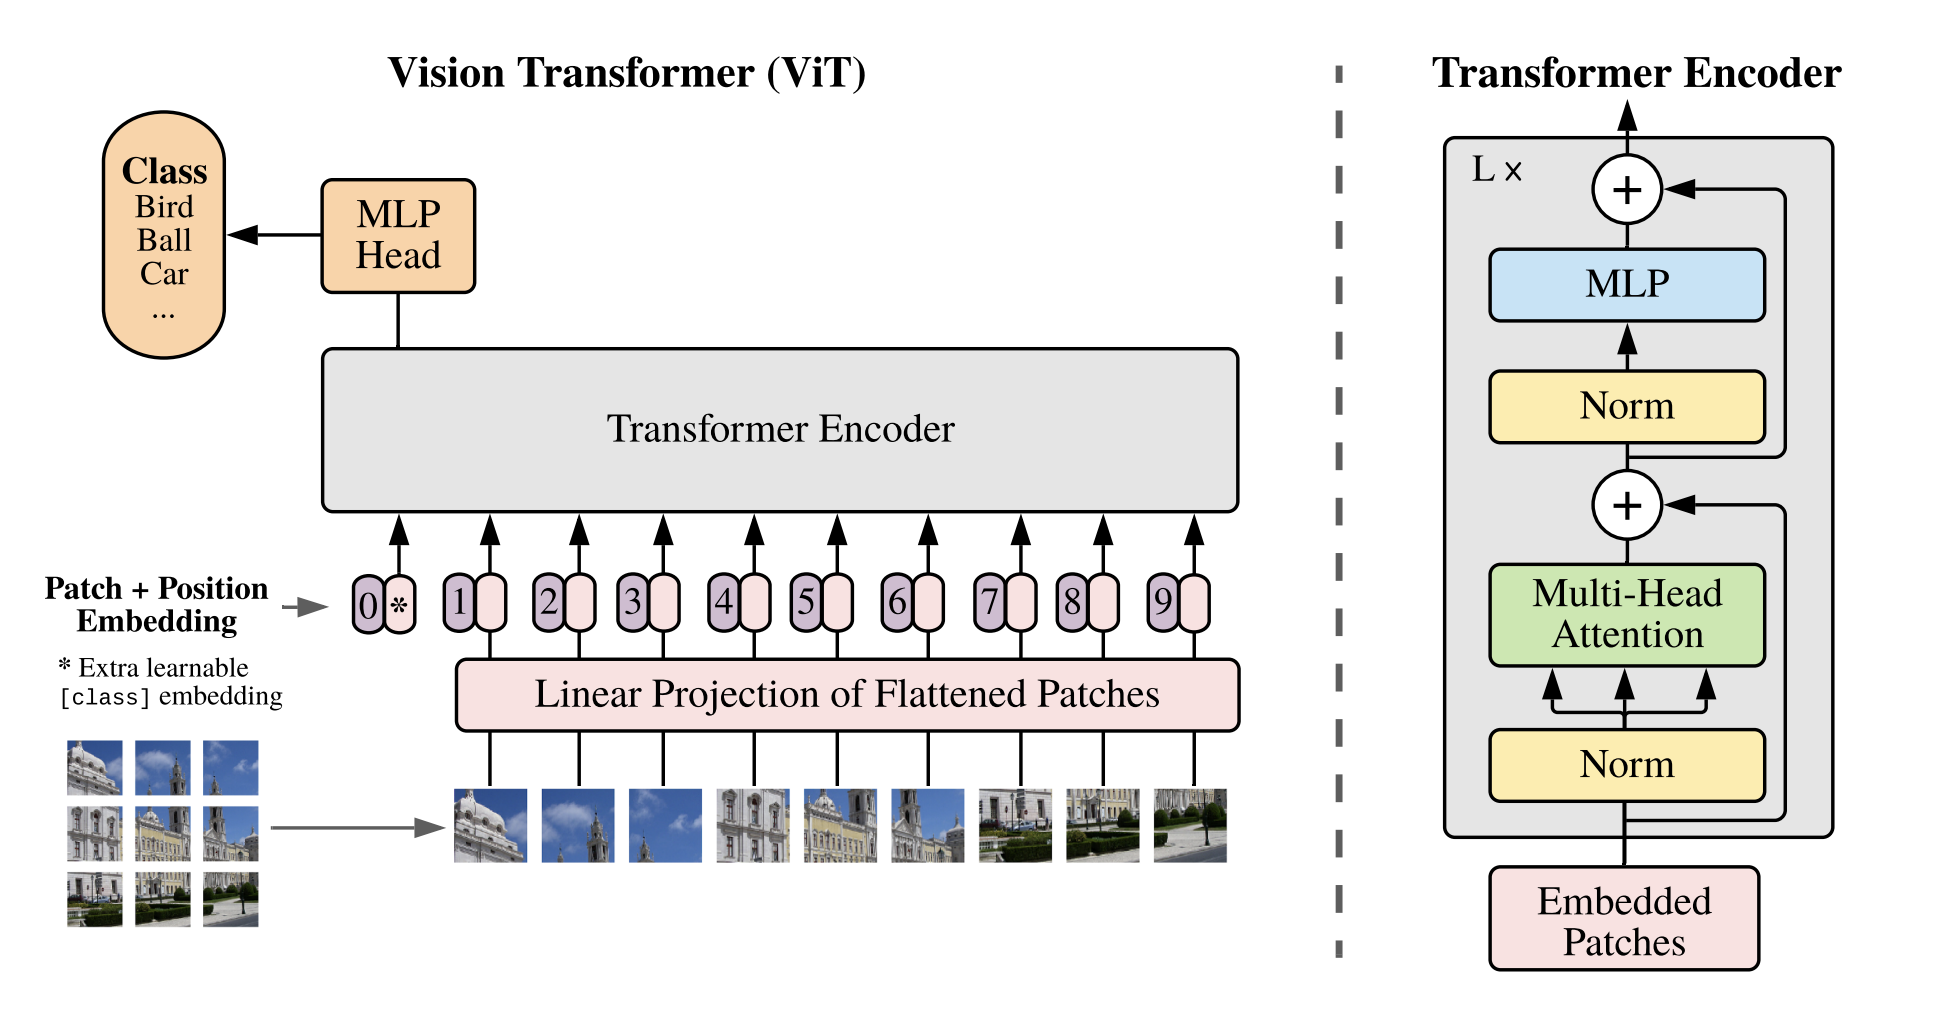
\includegraphics[width=0.8\textwidth]{images/appendix/vision_transformer/architecture.png}
    \caption{Vision Transformer (ViT) architecture \cite{vision_transformer}. The first patch + position embedding is the CLS token (classification token) which is used for image classification (its value is changed when the model learns to classify images).}
\end{figure}

\textbf{Patch embeddings:} The input image is divided into fixed-size non-overlapping patches (often 16x16). Each patch is flattened into a 1D (which has 16x16x3 = 768 values, for the RGB channels) vector and then linearly transformed (\texttt{nn.Linear()}) into a fixed-size vector of dimension $D$ (like tokens in NLP transform into embeddings) by \textbf{linear projection}:

\[ \text{Projected} = \text{FlattenPatch} \times W + b \]

\textbf{Position embeddings:} In order to let the transformer know the position of each patch spatially, positional embeddings are used: each patch 0, 1, ... is numbered (from top-left to bottom-right, rasterized) and then each position is embedded using sinusoidal position embedding, like we discussed in \ref{subsec:sinusoidal_embeddings}.

\textbf{Combining the embeddings:} The patch embeddings and the positional embeddings are \textbf{summed together} element-wise (\textbf{and not concatenated}, channel-wise) to form the input to the encoder.

\textbf{Transformer encoder:} The patch embeddings + positional embeddings are fed to the transformer encoder. It uses self-attention to weight the importance of each patch embedding in order to capture long-range relationships between patches.

\textbf{Classification head:} An MLP layer is used to classify the image after the encoder.

Overall, ViT uses self-attention to model relationships across all patches in an image, and because of the scalable nature of transformers, it providing an effective alternative to CNNs in vision tasks. Its success has created new ways of using transformers in image and video synthesis model.
